\documentclass[11pt,letterpaper]{article}

% Load some basic packages that are useful to have
% and that should be part of any LaTeX installation.
%
% be able to include figures
\usepackage{graphicx}
% get nice colors
\usepackage{xcolor}

% change default font to Palatino (looks nicer!)
\usepackage{apjfonts}
% load some useful math symbols/fonts
\usepackage{latexsym,amsfonts,amsmath,amssymb}

% comfort package to easily set margins
\usepackage[top=1in, bottom=1in, left=1in, right=1in]{geometry}

% control some spacings
%
% spacing after a paragraph
\setlength{\parskip}{.15cm}
% indentation at the top of a new paragraph
\setlength{\parindent}{0.0cm}


\begin{document}

\begin{center}
\Large
{\bf Ay190 -- Worksheet 7} \\
\large
Xiangcheng Ma \\
Date: \today
\end{center}

\section*{Measuring $\pi$ with an MC Experiment}
The MC estimate of $\pi$ with increasing number of points, $N$, is tabulated in Table~\ref{tb1}. The absolute error versus $\sqrt{N}$ is plotted in Figure~\ref{fig1}. The error basically follows $\sim 1/\sqrt{N}$ for not too large $N$. There is a threshold above which the error cannot be reduced by increasing $N$.
\begin{table}[h]
\centering
\begin{tabular}{ccccc}
\hline\hline
$n$ & $x_n$ & $(1/3)^n$ & absolute error & relative error \\
\hline
0 & 1.0 & 1.0 & 0.0 & 0.0 \\
1 & 0.333333 & 0.333333333333 & 9.93410748107e-09 & 2.98023224432e-08 \\
2 & 0.111111 & 0.111111111111 & 5.29819064732e-08 & 4.76837158259e-07 \\
3 & 0.0370373 & 0.037037037037 & 2.16342784749e-07 & 5.84125518823e-06 \\
4 & 0.0123466 & 0.0123456790123 & 8.71809912319e-07 & 7.06166028978e-05 \\
5 & 0.00411871 & 0.00411522633745 & 3.48814414362e-06 & 0.0008476190269 \\
6 & 0.00138569 & 0.00137174211248 & 1.39522571909e-05 & 0.0101711954921 \\
7 & 0.000513056 & 0.000457247370828 & 5.58089223023e-05 & 0.122054113075 \\
8 & 0.000375651 & 0.000152415790276 & 0.000223235614917 & 1.46464886947 \\
9 & 0.000943748 & 5.08052634253e-05 & 0.000892942551319 & 17.5757882376 \\
10 & 0.00358871 & 1.69350878084e-05 & 0.00357177023583 & 210.909460655 \\
11 & 0.0142927 & 5.64502926948e-06 & 0.0142870812639 & 2530.91358466 \\
12 & 0.0571502 & 1.88167642316e-06 & 0.0571483257835 & 30370.9634027 \\
13 & 0.228594 & 6.27225474386e-07 & 0.228593318278 & 364451.584977 \\
14 & 0.914374 & 2.09075158129e-07 & 0.914373307961 & 4373419.18641 \\
15 & 3.65749 & 6.96917193763e-08 & 3.6574932832 & 52481030.9737 \\
\hline\hline
\end{tabular}
\label{tb1}
\caption{An Unstable Calculation}
\end{table}


\begin{figure}[ht]
\centering
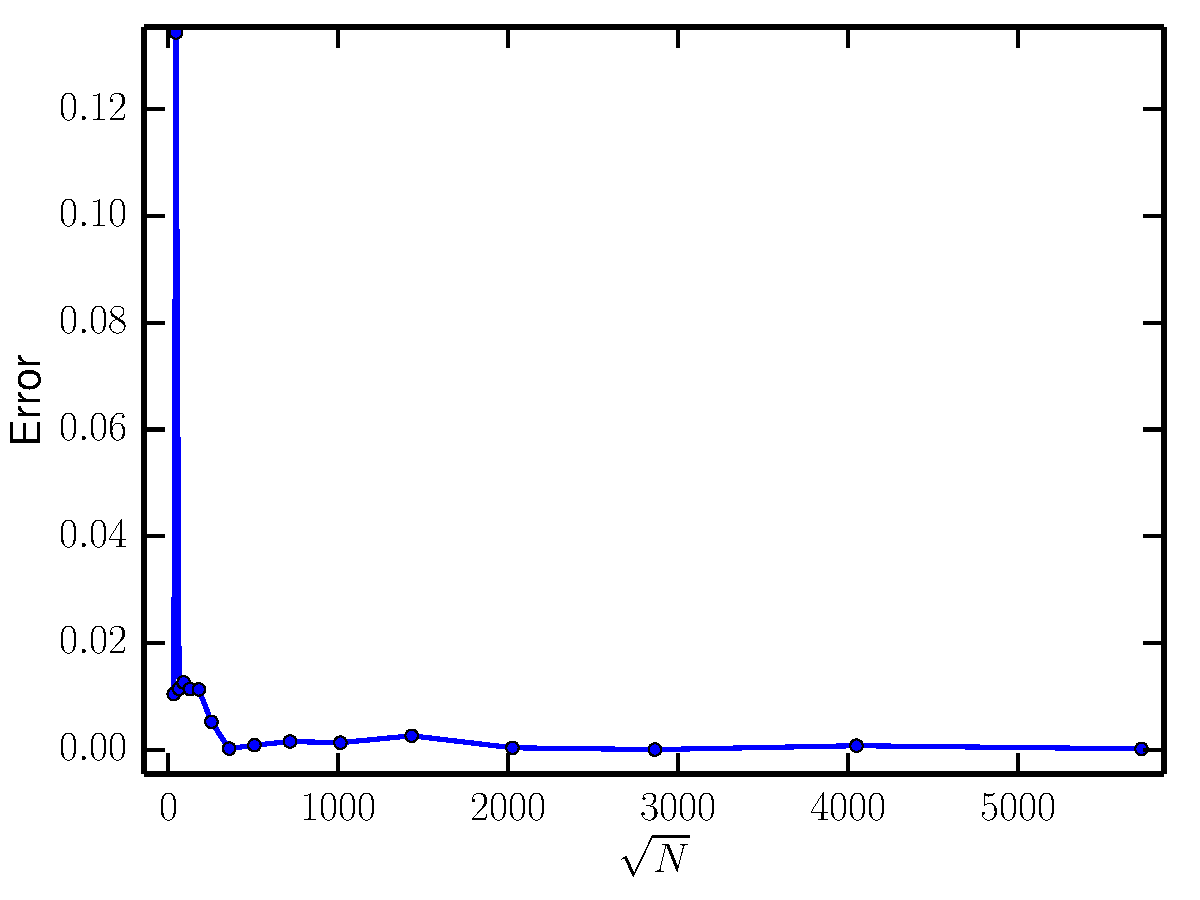
\includegraphics[width=0.5\textwidth]{fig1.pdf}
\caption{MC Estimation of $\pi$}
\label{fig1}
\end{figure}


\section*{The Birthday Paradox}
For number of people $N$, recall that there are 365 days in a year, the probability that at least two of them have same birthday is 
\begin{equation}
 P = 1 - \frac{365!/(365-N)!}{365^N} ,
\end{equation}	
where the bulk after the minus sign is just the probability that all of them have different birthdays.

WIth MC method, for each $N$, I do 20000 experiments and get an estimated probability as tabulated below.
\begin{table}[h]
\centering
\begin{tabular}{cc}
\hline\hline
$N$ & Probability \\
\hline
21 & 0.4473 \\
22 & 0.47475 \\
23 & 0.50775 \\
24 & 0.54095 \\
25 & 0.5763 \\
\hline\hline
\end{tabular}
\label{tb2}
\caption{Birthday Paradox}
\end{table}



\section*{MC Integration}
In this section, the intergration
\begin{equation}
  I = \int_2^3 f(x)~{\rm d}x = \int_2^3 x^2+1~{\rm d}x = \frac{22}{3}
\end{equation}
will be calculated using MC method.

The results are tabulated in the following table and the error as a function of $\sqrt{N}$ is plotted in Figure~\ref{fig2}. As in question 1, the error basically follows $\sim 1/\sqrt{N}$ for not too large $N$. There is a threshold above which the error cannot be reduced by increasing $N$.
\begin{figure}[ht]
\centering
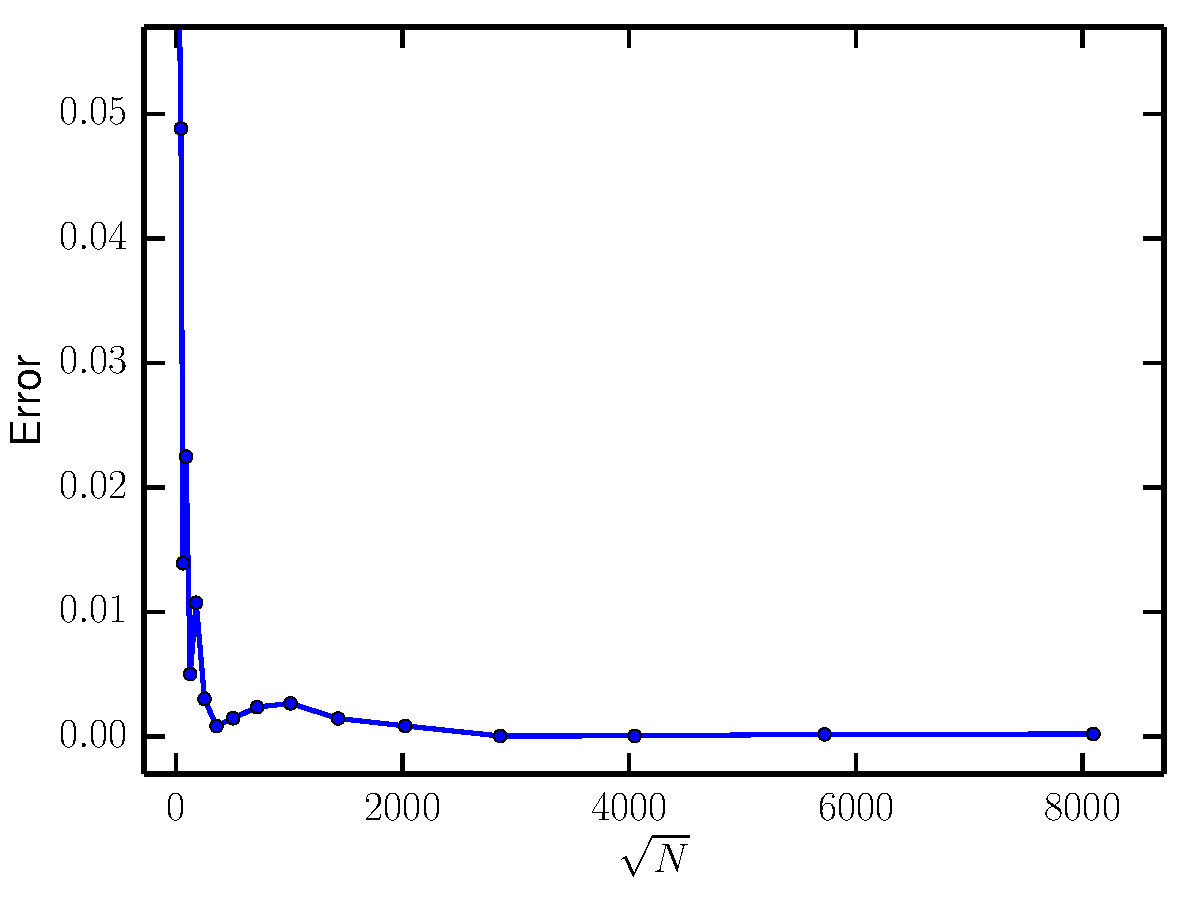
\includegraphics[width=0.5\textwidth]{fig2.pdf}
\caption{MC Estimation of $\pi$}
\label{fig2}
\end{figure}

\end{document}
